\documentclass{article}
\usepackage[spanish]{babel}
\usepackage[utf8]{inputenc}
\usepackage[T1]{fontenc}
\usepackage{hyperref}
\usepackage{xcolor}
\usepackage{listings}
\usepackage{minted}
\usepackage{graphicx}
\usepackage{longtable}
\usepackage{multirow}
\hypersetup{
    colorlinks,
    linkcolor={red!50!black},
    citecolor={blue!50!black},
    urlcolor={blue!80!black}
}

\title{P3: Rendimiento web}
\author{Daniel Ramos}
\date{\today}

\begin{document}

\maketitle

\begin{center}
    \large Herramientas HTML y CSS I
\end{center}

\newpage

\tableofcontents

\newpage

\section*{Introducción}

Este informe recoge el proceso de análisis y mejora del rendimiento web aplicado al proyecto desarrollado en las prácticas anteriores del curso. El objetivo principal ha sido optimizar la experiencia de usuario mediante una reducción significativa de los tiempos de carga y una mejora en las métricas clave de rendimiento.

Para ello, se ha realizado una evaluación técnica detallada del estado inicial del sitio utilizando herramientas como las DevTools del navegador y Google PageSpeed Insights. A partir de los resultados obtenidos, se han aplicado una serie de cambios progresivos —desde mejoras básicas como el uso de \textit{lazy loading} y carga asíncrona de scripts, hasta optimizaciones más avanzadas como la fachada para vídeos o el recorte y dimensionado específico de imágenes— con el fin de reducir la cantidad de recursos críticos en la carga inicial.

El documento está estructurado en varias secciones que reflejan el desarrollo completo del trabajo: análisis comparativos del tiempo de carga, descripción técnica de los cambios aplicados, informe de mejoras basadas en las sugerencias automáticas de Google PageSpeed Insights y una reflexión final sobre las decisiones adoptadas.

Además, se incluyen enlaces al repositorio del proyecto y a la versión desplegada del sitio web:

\begin{itemize}
    \item \href{https://github.com/DanielRamosAcosta/hhyc-dramosac}{Repositorio en GitHub}
    \item \href{https://www.danielramos.me/hhyc-dramosac}{Página web desplegada}
\end{itemize}

\newpage

\section{Análisis del tiempo de carga}\label{sec:analisis-de-tiempo-de-carga}

Con el objetivo de evaluar el rendimiento de la web desarrollada, se han realizado tres análisis consecutivos del tiempo de carga, cada uno asociado a una fase distinta del proceso de optimización.

El primer análisis se llevó a cabo sobre la versión original del sitio, sin mejoras específicas de rendimiento. Posteriormente, se aplicaron técnicas básicas como el \textit{lazy loading} de imágenes y la carga diferida de scripts, tras lo cual se repitió la medición. Finalmente, se implementaron las recomendaciones de PageSpeed Insights, lo que permitió realizar un tercer y último análisis comparativo.

En los siguientes apartados se presenta cada análisis individual, seguido de una tabla comparativa conjunta que resume los resultados obtenidos y el impacto real de las mejoras aplicadas.

\subsection{Primer análisis (estado inicial)}\label{subsec:primer-analisis}

\begin{longtable}{c|c|c|c|c|c}
    \hline
    \textbf{TI} & \textbf{UR} & \textbf{TC} & \textbf{PT} & \textbf{PR} & \textbf{CR} \\
    \endhead
    \hline
    Inicio & \href{https://www.danielramos.me/hhyc-dramosac/index.html}{index.html} & 34,81s & 5812,8 Kb & 4951,36 Kb & 30 \\
    Recetas & \href{https://www.danielramos.me/hhyc-dramosac/recipes.html}{recipes.html} & 7,12s & 796 Kb & 618 Kb & 27 \\
    Escaldón & \href{https://www.danielramos.me/hhyc-dramosac/recipes-escaldon.html}{recipes-escaldon.html} & 20,7s & 4843,52 Kb & 2007,04 Kb & 46 \\
    Batata & \href{https://www.danielramos.me/hhyc-dramosac/recipes-batata.html}{recipes-batata.html} & 17,54s & 4485,12 Kb & 1648,64 Kb & 47 \\
    Enlaces & \href{https://www.danielramos.me/hhyc-dramosac/links.html}{links.html} & 631,2ms & 74 Kb & 50 Kb & 14 \\
    \hline
     \\[1.5ex]
     \caption{
          Ejemplos de imágenes optimizadas.
          Leyenda: 
          \textbf{TI}: Título de la página, 
          \textbf{UR}: URL, 
          \textbf{TC}: Tiempo de carga (promedio) 
          \textbf{PT}: Peso total 
          \textbf{PR}: Peso transferido, 
          \textbf{CR}: Cantidad de recursos que contine la página.
     }
    \label{tab:imagenes-optimizadas}
\end{longtable}

\subsection{Segundo análisis (tras aplicar \textit{lazy loading} y \texttt{defer})}\label{sec:segundo-analisis}

\begin{longtable}{c|c|c|c|c|c}
    \hline
    \textbf{TI} & \textbf{UR} & \textbf{TC} & \textbf{PT} & \textbf{PR} & \textbf{CR} \\
    \endhead
    \hline
    Inicio & \href{https://www.danielramos.me/hhyc-dramosac/index.html}{index.html} & 28,43s & 4812,8 Kb & 4751,36 Kb & 30 \\
    Recetas & \href{https://www.danielramos.me/hhyc-dramosac/recipes.html}{recipes.html} & 5,43s & 555 Kb & 541 Kb & 27 \\
    Escaldón & \href{https://www.danielramos.me/hhyc-dramosac/recipes-escaldon.html}{recipes-escaldon.html} & 16,1s & 4362,24 Kb & 1525,76 Kb & 46 \\
    Batata & \href{https://www.danielramos.me/hhyc-dramosac/recipes-batata.html}{recipes-batata.html} & 14,41s & 4167,68 Kb & 1331,2 Kb & 47 \\
    Enlaces & \href{https://www.danielramos.me/hhyc-dramosac/links.html}{links.html} & 527ms & 51,9 Kb & 43,72 Kb & 14 \\
    \hline
     \\[1.5ex]
     \caption{
          Ejemplos de imágenes optimizadas.
          Leyenda: 
          \textbf{TI}: Título de la página, 
          \textbf{UR}: URL, 
          \textbf{TC}: Tiempo de carga (promedio) 
          \textbf{PT}: Peso total 
          \textbf{PR}: Peso transferido, 
          \textbf{CR}: Cantidad de recursos que contine la página.
     }
    \label{tab:imagenes-optimizadas}
\end{longtable}

\subsection{Tercer análisis (tras aplicar mejoras propuestas)}\label{sec:tercer-analisis}

\begin{longtable}{c|c|c|c|c|c}
    \hline
    \textbf{TI} & \textbf{UR} & \textbf{TC} & \textbf{PT} & \textbf{PR} & \textbf{CR} \\
    \endhead
    \hline
    Inicio & \href{https://www.danielramos.me/hhyc-dramosac/index.html}{index.html} & 25,5s & 2396,16 Kb & 2293,76 Kb & 30 \\
    Recetas & \href{https://www.danielramos.me/hhyc-dramosac/recipes.html}{recipes.html} & 4,42s & 482 Kb & 455 Kb & 27 \\
    Escaldón & \href{https://www.danielramos.me/hhyc-dramosac/recipes-escaldon.html}{recipes-escaldon.html} & 2,3s & 223 Kb & 199 Kb & 46 \\
    Batata & \href{https://www.danielramos.me/hhyc-dramosac/recipes-batata.html}{recipes-batata.html} & 1,6s & 175 Kb & 151 Kb & 47 \\
    Enlaces & \href{https://www.danielramos.me/hhyc-dramosac/links.html}{links.html} & 623ms & 62 Kb & 42 Kb & 14 \\
    \hline
     \\[1.5ex]
     \caption{
          Ejemplos de imágenes optimizadas.
          Leyenda: 
          \textbf{TI}: Título de la página, 
          \textbf{UR}: URL, 
          \textbf{TC}: Tiempo de carga (promedio) 
          \textbf{PT}: Peso total 
          \textbf{PR}: Peso transferido, 
          \textbf{CR}: Cantidad de recursos que contine la página.
     }
    \label{tab:pagespeed-insights}
\end{longtable}

\subsection{Comparativa y análisis de resultados}\label{sec:comparativa-y-analisis-de-resultados}

Al comparar los tres análisis de carga realizados, se observa una mejora progresiva en el rendimiento general de la página web.

Entre el primer análisis (estado inicial) y el segundo (tras aplicar \textit{lazy loading} y carga asíncrona de scripts), el tiempo de carga disminuyó ligeramente —en torno a 6 segundos en algunos casos— debido principalmente a que las imágenes fuera del \textit{viewport} dejaron de cargarse de forma inmediata, y los scripts no críticos pasaron a cargarse de forma diferida mediante el atributo \texttt{defer}.

Sin embargo, la mejora más significativa se produjo entre el segundo y el tercer análisis (tras aplicar las recomendaciones de PageSpeed Insights), donde se observaron reducciones de hasta 12 segundos adicionales. Esta mejora se debe en gran parte al mejorar el rendimiento de la carga de los vídeos, que más adelante se detallará.

Este análisis refleja la importancia de aplicar estrategias de optimización en el desarrollo web. A través de ajustes relativamente sencillos se ha logrado reducir el tiempo de carga hasta en 18 segundos en los casos más críticos, mejorando considerablemente la experiencia de usuario y la eficiencia del sitio.

\section{Primeros cambios}\label{sec:primeros-cambios}

\subsection{Aplicación de \texttt{loading="lazy"} en imágenes}\label{subsec:loading-lazy}

Se ha realizado un análisis en todas las páginas del sitio para identificar las imágenes que no aparecen en el \textit{viewport} durante la carga inicial. A todas aquellas que no forman parte del contenido visible inmediatamente se les ha aplicado el atributo \texttt{loading="lazy"}.

Este atributo permite al navegador posponer la descarga de dichas imágenes hasta que el usuario haga scroll y se acerque a su posición en la página. De esta forma, se reduce la cantidad de recursos cargados de forma anticipada, lo cual disminuye el tiempo de carga inicial y mejora el rendimiento general del sitio.

\subsection{Uso de \texttt{defer} en scripts}\label{subsec:defer-en-scripts}

En este proyecto, la carga de scripts no representaba un gran impacto en el rendimiento, ya que no se utilizan archivos JavaScript especialmente pesados. Aun así, se han aplicado mejoras para optimizar su carga.

Concretamente, se ha añadido el atributo \texttt{defer} a todos los scripts que no eran críticos para el renderizado inicial de la página. Este atributo permite que los scripts se descarguen en paralelo durante la carga del HTML, pero se ejecuten únicamente una vez que el árbol DOM esté completamente construido.

Se optó por \texttt{defer} en lugar de otras opciones como \texttt{async}, ya que todos los scripts dependen de elementos del DOM —ya sea para leerlos o para añadirles eventos—, por lo que es necesario que el DOM esté completamente cargado antes de su ejecución.

\section{Informe de mejoras}\label{sec:informe-de-mejoras}

\subsection{Resultados del test inicial (PageSpeed Insights)}\label{subsec:resultados-del-test-inicial}

El análisis inicial realizado con Google PageSpeed Insights reveló varios problemas de rendimiento en las páginas del sitio web.

\begin{figure}[h!]
    \centering
    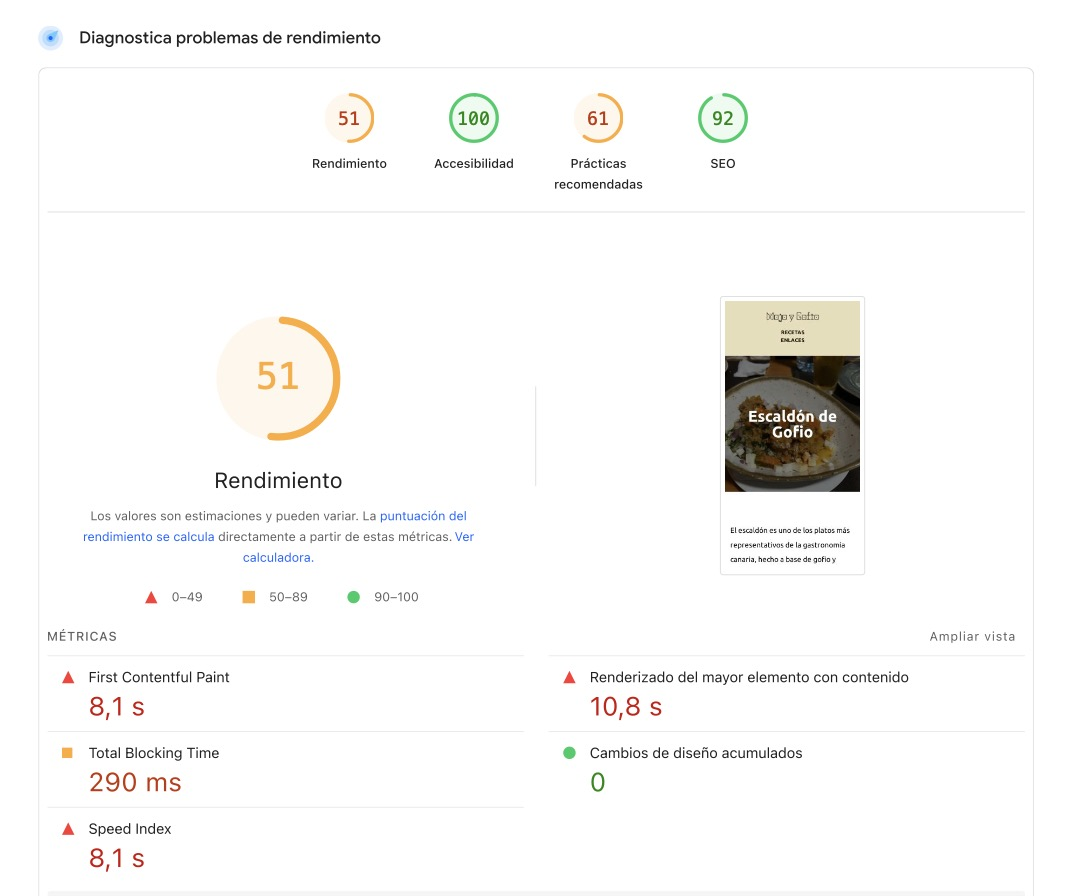
\includegraphics[width=0.8\textwidth]{./img/p3/escaldon-performance-before}
    \caption{Puntuación de la página de detalle del escaldón antes de las mejoras.}
    \label{fig:escaldon-performance-before}
\end{figure}

Entre las observaciones más relevantes se encontraban:

\begin{itemize}
    \item Carga sin optimizar de recursos de terceros, que podrían diferirse mediante técnicas como el uso de una fachada.
    \item Presencia de código JavaScript no utilizado, especialmente relacionado con la carga de vídeos.
    \item Uso de imágenes con una resolución mayor a la necesaria para su visualización efectiva.
\end{itemize}

Además, se detectaron otras advertencias menores, como recomendaciones sobre el almacenamiento en caché de recursos, las cuales no se pudieron abordar directamente por las limitaciones del entorno de despliegue (GitHub Pages).

Una de las métricas que presentaba un valor especialmente bajo era el \textit{Largest Contentful Paint} (LCP), es decir, el tiempo de renderizado del mayor elemento con contenido. Aunque la imagen principal no tardaba demasiado en descargarse, sí se demoraba su renderizado. Tras analizar el problema, se identificó que otros elementos estaban bloqueando el renderizado de la imagen de cabecera.

En este análisis se detectó también que se estaban cargando dos familias tipográficas desde Google Fonts: Sankofa para el logotipo y Ubuntu para el resto del contenido. Además, ambas fuentes se estaban importando con todos sus pesos disponibles, lo que incrementaba considerablemente la cantidad de recursos a descargar y afectaba negativamente a las métricas de rendimiento.

La puntuación de rendimiento fue especialmente baja en las páginas de detalle de las recetas, con un valor aproximado de 50 en versión móvil. En cambio, las páginas de índice y listados de recetas obtuvieron puntuaciones iniciales más elevadas, en torno a 80.

\subsection{Cambios realizados en base a sugerencias}\label{subsec:cambios-realizados}

A partir del análisis inicial con PageSpeed Insights, se implementaron una serie de mejoras orientadas a reducir los tiempos de carga y mejorar las métricas clave de rendimiento.

\begin{itemize}
    \item \textbf{Optimización de fuentes tipográficas:} Se eliminó la carga de la fuente Sankofa, ya que el logotipo fue convertido a un elemento \texttt{SVG}. Además, se limitó la carga de la fuente Ubuntu únicamente a los pesos utilizados en la web, reduciendo así el número de solicitudes y el tamaño total de los archivos CSS generados por Google Fonts.
    
    \item \textbf{Ajuste de tamaños en imágenes \texttt{srcset}:} Se revisaron los atributos \texttt{srcset} de las imágenes para asegurar que incluyeran resoluciones acordes a los tamaños reales de visualización. Esto permitió evitar la descarga de imágenes innecesariamente grandes. Gracias a la herramienta \texttt{sharp}, se generaron versiones intermedias de forma eficiente.

    \item \textbf{Recorte de imágenes verticales a proporción 16:9:} Algunas imágenes originalmente en formato vertical fueron recortadas a una proporción horizontal 16:9, en consonancia con el diseño final de la web. Esto redujo el peso visual y mejoró la percepción del contenido por parte del usuario.

    \item \textbf{Definición de dimensiones en imágenes:} Se especificaron explícitamente los atributos \texttt{width} y \texttt{height} en las imágenes que lo permitían. Esto contribuye a evitar los saltos de contenido (\textit{layout shifts}) durante la carga de la página, lo cual tiene un impacto positivo en métricas como el \textit{Cumulative Layout Shift} (CLS).

    \item \textbf{Carga diferida de vídeos mediante fachada:} Uno de los cambios con mayor impacto fue sustituir el \texttt{iframe} de YouTube por una fachada estática. Al insertar directamente el \texttt{iframe}, se cargan automáticamente varios recursos JavaScript de YouTube, lo que ralentiza significativamente la carga inicial. En su lugar, se implementó una fachada consistente en una imagen del vídeo con un botón de reproducción superpuesto. El vídeo solo se carga cuando el usuario hace clic, momento en el que se inserta dinámicamente el \texttt{iframe} real. Esta técnica redujo de forma notable la cantidad de scripts cargados en el arranque.

    \item \textbf{Preload de imágenes críticas:} Se han añadido etiquetas \texttt{<link rel="preload">} para las imágenes que aparecen en el \textit{viewport} durante la carga inicial de la página. Esta técnica indica al navegador que debe priorizar la descarga de estos recursos incluso antes de que se encuentren en el árbol del DOM mediante elementos \texttt{<img>}, permitiendo así una carga más eficiente y acelerando el \textit{Largest Contentful Paint}.

\end{itemize}


\subsection{Resultados tras las mejoras}\label{subsec:resultados-tras-las-mejoras}

En la Tabla~\ref{tab:pagespeed-insights} se pueden observar las mejoras significativas obtenidas en las métricas de rendimiento tras aplicar los cambios propuestos.

Aunque no se dispone de un desglose detallado por métrica en este informe, durante el proceso de desarrollo se identificó que la mejora más notable en tiempo de carga se produjo al implementar la técnica de la fachada para el vídeo de YouTube. Esta optimización evitó la carga inmediata del \texttt{iframe} y los recursos asociados, lo que tuvo un impacto muy positivo en el \textit{Largest Contentful Paint} y en el número total de recursos descargados durante la carga inicial.

Adicionalmente, la optimización de fuentes —eliminando Sankofa y reduciendo los pesos de Ubuntu— también contribuyó a mejorar el \textit{First Contentful Paint} y reducir el tiempo hasta la interactividad.

Gracias a estas medidas, la puntuación promedio de rendimiento obtenida en PageSpeed Insights mejoró de 72 a 92, lo cual se considera un resultado sólido dentro del rango óptimo.

A pesar de estas mejoras, quedaron algunos puntos pendientes de resolver. Por ejemplo, todas las páginas (excepto \texttt{links.html}) muestran al menos una imagen dentro del \textit{viewport} al cargar, lo cual PageSpeed Insights sugiere evitar para lograr tiempos aún más bajos en la carga inicial. Sin embargo, en el contexto de este proyecto, mostrar contenido visual inmediato se considera prioritario para la experiencia del usuario. Además, como se especificaba en las prácticas anteriores que debía incluirse una imagen de cabecera, y dado que cambiar esta decisión afectaría al diseño general del sitio, se ha optado conscientemente por mantener esta estructura.

\begin{figure}[h!]
    \centering
    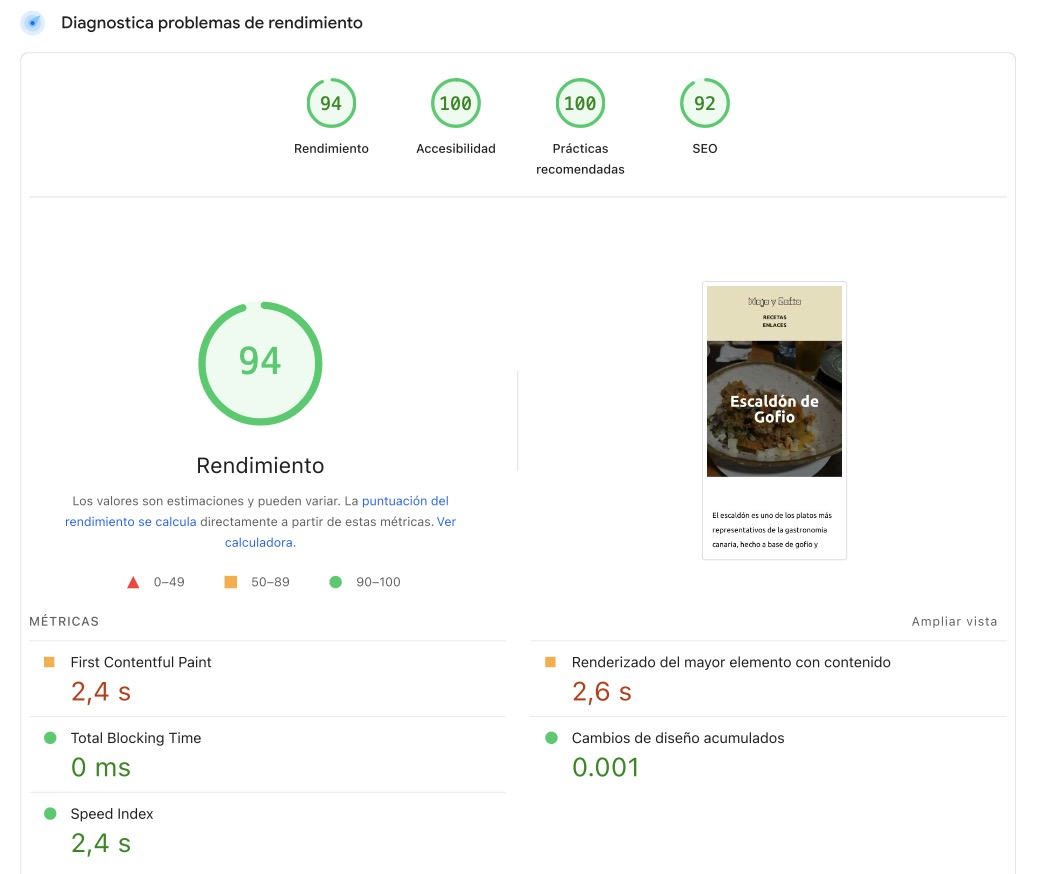
\includegraphics[width=0.8\textwidth]{./img/p3/escaldon-performance-after}
    \caption{Puntuación de la página de detalle del escaldón después de las mejoras.}
    \label{fig:escaldon-performance-after}
\end{figure}

\section{Preguntas finales}\label{sec:preguntas-finales}

Al aplicar \textit{lazy loading} a las imágenes, se observa en la pestaña de red de las herramientas para desarrolladores que las imágenes fuera del \textit{viewport} ya no se cargan durante la carga inicial de la página. En su lugar, su descarga se difiere hasta que el usuario hace \textit{scroll} hacia su posición.

Esto reduce el número de peticiones HTTP iniciales, disminuye la cantidad de datos transferidos y mejora notablemente métricas como el \textit{Largest Contentful Paint} y el \textit{Time to Interactive}. Además, reduce la carga en dispositivos con conexiones lentas o recursos limitados.

\subsection{Impacto y posibles problemas del uso de \texttt{defer}}\label{subsec:impacto-y-problemas-de-defer}

Al aplicar el atributo \texttt{defer} a los scripts, estos se descargan en paralelo mientras se parsea el HTML, pero su ejecución se difiere hasta que el DOM está completamente construido. Esto permite evitar bloqueos en el renderizado y mejora el tiempo de carga percibido.

Por el contrario, el uso de \texttt{async} puede provocar problemas, ya que los scripts se ejecutan tan pronto como terminan de descargarse, sin esperar al DOM ni garantizar el orden de ejecución. Esto puede resultar en errores si los scripts intentan acceder a elementos que aún no existen.

En el caso de esta web en particular, todos los scripts interactúan con el DOM en el momento de cargarse (por ejemplo, añadiendo eventos o accediendo a nodos). Por ello, es imprescindible el uso de \texttt{defer} para evitar errores como el acceso a nodos inexistentes durante la ejecución.

\subsection{Carga asíncrona de estilos: \textquestiondown es viable?}\label{subsec:carga-asincrona-de-estilos}

La carga asíncrona de hojas de estilo es técnicamente posible mediante técnicas como \texttt{media="print"} o \texttt{rel="preload"} seguido de su activación mediante JavaScript. Sin embargo, estas prácticas implican ciertos riesgos.

El principal inconveniente es la posibilidad de un \textit{flash of unstyled content} (FOUC), en el que el usuario visualiza el contenido sin estilos aplicados durante un breve instante. Esto puede generar una experiencia negativa y una percepción de baja calidad.

Por este motivo, en este proyecto no se ha aplicado carga asíncrona a las hojas de estilo principales. No obstante, sí se ha optado por cargar de forma asíncrona las hojas de estilo de las fuentes tipográficas. En este caso concreto, se ha considerado aceptable un posible \textit{flash of unstyled text} (FOUT), ya que se han definido buenos \textit{fallbacks} tipográficos y el impacto visual es mínimo. Esta decisión permite optimizar el rendimiento sin comprometer gravemente la estética del sitio.

\end{document}
